\documentclass[aspectratio=169, 12pt]{beamer}

% ---- Theme ----
\usetheme{Madrid}
\usecolortheme{seahorse}
\setbeamertemplate{navigation symbols}{}
\setbeamertemplate{footline}[frame number]
\setbeamerfont{frametitle}{size=\large, series=\bfseries}

% ---- Packages ----
\usepackage{graphicx}
\usepackage{booktabs}
\usepackage{tikz}
\usepackage{xcolor}
\usepackage{hyperref}
\usepackage{fontenc}

% ---- Custom colors ----
\definecolor{classical}{HTML}{4A90D9}
\definecolor{dlred}{HTML}{E85D75}
\definecolor{goodgreen}{HTML}{2ECC71}
\definecolor{badred}{HTML}{E74C3C}
\definecolor{darkgray}{HTML}{333333}

% ---- Image path ----
\graphicspath{{../visuals/}}

% ---- Title ----
\title{\textbf{Classical vs.\ Deep Learning Agent}\\for Autonomous Driving}
\subtitle{CarRacing-v3 --- Gymnasium Box2D}
\author{Yue Wu}
\date{April 2026}

\begin{document}

% ==========================================================
% SLIDE 1: Title
% ==========================================================
\begin{frame}
\titlepage
\end{frame}

% ==========================================================
% SLIDE 2: Motivation
% ==========================================================
\begin{frame}{Motivation: Why Autonomous Driving?}
\textbf{Driving is one of the highest-stakes decision tasks humans do every day.}\\[0.3em]
A self-driving system has to turn raw sensor data into safe, real-time control --- tens of times per second, with no room for failure.

\vspace{0.6em}
It's also a \textbf{canonical AI problem} because it stitches together three classically hard sub-problems:
\begin{itemize}\setlength\itemsep{0.2em}
    \item \textbf{Perception:} where is the road, the lane, the other agents?
    \item \textbf{Planning:} where should the car go next?
    \item \textbf{Control:} how much steering, gas, brake to get there?
\end{itemize}

\vspace{0.6em}
\textbf{CarRacing-v3} is the smallest toy version of this problem that still has all three pieces. Top-down view of a randomly generated track, 96$\times$96 pixels in, steer/gas/brake out. Simple enough to solve in a class project --- complex enough that \textit{how} you solve it matters.
\end{frame}

% ==========================================================
% SLIDE 3: The Task
% ==========================================================
\begin{frame}{The Task: CarRacing-v3}
\begin{columns}[T]
\begin{column}{0.55\textwidth}
\textbf{Goal:} Drive a car around a randomly generated racetrack.

\vspace{0.3em}
\textbf{Input:} 96$\times$96 RGB pixel image each frame

\textbf{Output:} 3 continuous numbers --- steer, gas, brake

\vspace{0.3em}
\textbf{Reward:}
\begin{itemize}\setlength\itemsep{0.1em}
    \item $+1000/N$ per road tile visited ($N =$ total tiles)
    \item $-0.1$ per frame (penalizes slow driving)
    \item Perfect lap $\approx$ 900+
\end{itemize}

\vspace{0.3em}
\textbf{The twist:} Build \textbf{two agents} that solve the same task in completely different ways, then compare.
\end{column}
\begin{column}{0.42\textwidth}
\centering
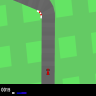
\includegraphics[width=0.85\textwidth]{game_screenshot.png}

\vspace{0.3em}
{\small\color{gray} Top-down view --- car at center-bottom}
\end{column}
\end{columns}
\end{frame}

% ==========================================================
% SLIDE 3: Two Approaches Overview
% ==========================================================
\begin{frame}{Two Approaches}
\centering
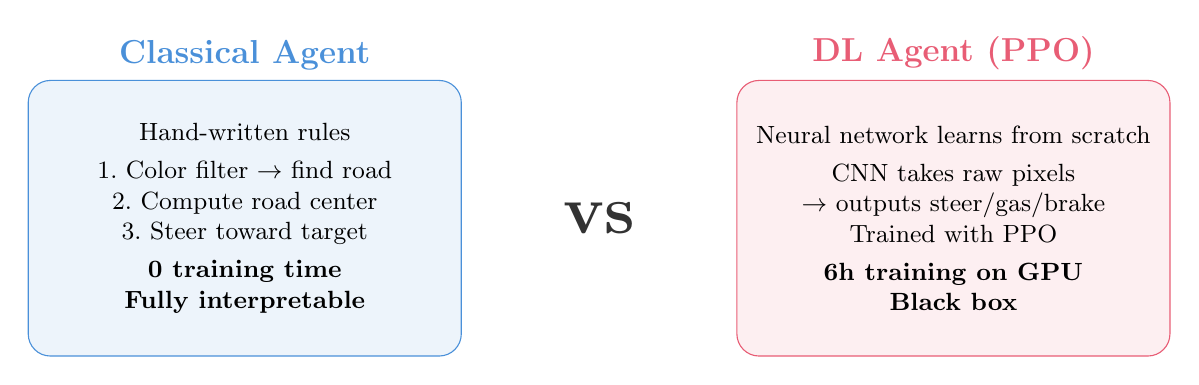
\begin{tikzpicture}
    % Classical box
    \node[draw=classical, fill=classical!10, rounded corners=8pt,
          minimum width=5.5cm, minimum height=3.5cm, align=center]
          (cls) at (-4.5, 0) {};
    \node[above, font=\large\bfseries, color=classical] at (cls.north) {Classical Agent};
    \node[align=center, font=\small] at (cls.center) {
        Hand-written rules\\[0.3em]
        1.\ Color filter $\to$ find road\\
        2.\ Compute road center\\
        3.\ Steer toward target\\[0.3em]
        \textbf{0 training time}\\
        \textbf{Fully interpretable}
    };

    % DL box
    \node[draw=dlred, fill=dlred!10, rounded corners=8pt,
          minimum width=5.5cm, minimum height=3.5cm, align=center]
          (dl) at (4.5, 0) {};
    \node[above, font=\large\bfseries, color=dlred] at (dl.north) {DL Agent (PPO)};
    \node[align=center, font=\small] at (dl.center) {
        Neural network learns from scratch\\[0.3em]
        CNN takes raw pixels\\
        $\to$ outputs steer/gas/brake\\
        Trained with PPO\\[0.3em]
        \textbf{6h training on GPU}\\
        \textbf{Black box}
    };

    % VS
    \node[font=\Huge\bfseries, color=darkgray] at (0, 0) {vs};
\end{tikzpicture}
\end{frame}

% ==========================================================
% SLIDE 4: Classical Perception Pipeline
% ==========================================================
\begin{frame}{Classical Agent --- Perception Pipeline}
\centering
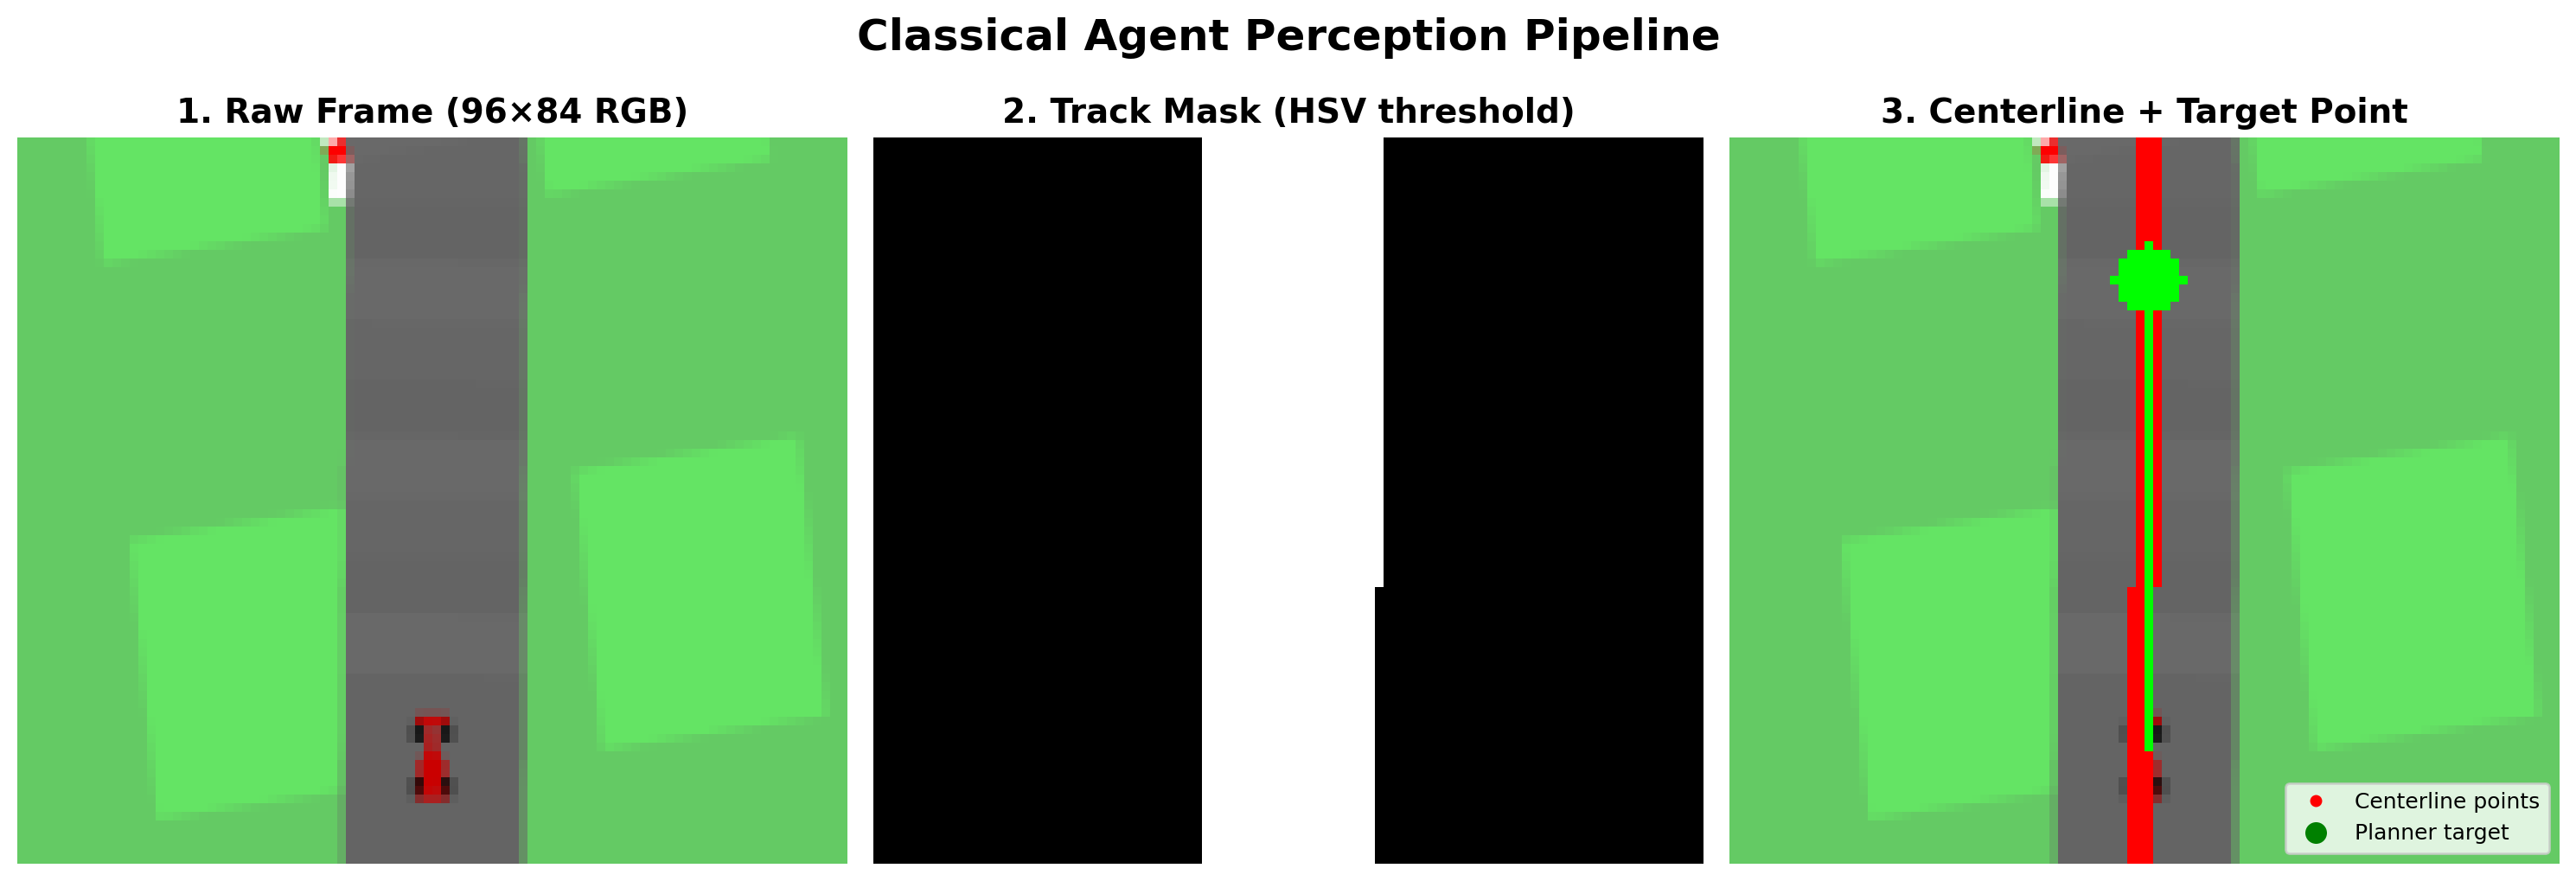
\includegraphics[width=0.95\textwidth]{perception_pipeline.png}

\vspace{0.5em}
\begin{enumerate}
    \item Convert image to HSV --- gray pixels have low saturation, grass has high
    \item Mark road pixels white (low color intensity = gray asphalt, or yellow stripe)
    \item For each row, find the middle of the white pixels $\to$ \textbf{centerline}
    \item Pick a target point ahead $\to$ steer toward it
\end{enumerate}
\end{frame}

% ==========================================================
% SLIDE 5: Classical Overview — Flow Diagram
% ==========================================================
\begin{frame}{Classical Agent --- Overview}
\begin{columns}[T]
\begin{column}{0.55\textwidth}
\vspace{1em}
Three stages, all hand-written rules:

\vspace{0.5em}
\begin{enumerate}\setlength\itemsep{0.5em}
    \item \textbf{Perception} --- find the road in the image and compute its center line (red dots in Panel 3)
    \item \textbf{Planning} --- pick a target point up the road to aim at (green dot in Panel 3)
    \item \textbf{Control} --- compute how much to steer, how much gas, how much brake
\end{enumerate}

\vspace{0.5em}
{\small Every decision is a named constant in the code --- fully interpretable, zero training.}
\end{column}
\begin{column}{0.42\textwidth}
\centering
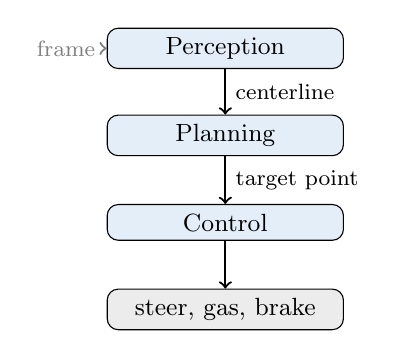
\begin{tikzpicture}[scale=0.85, every node/.style={font=\small}]
    \node[draw, rounded corners, fill=classical!15, minimum width=3cm] (perc) at (0,3.5) {Perception};
    \node[draw, rounded corners, fill=classical!15, minimum width=3cm] (plan) at (0,2.2) {Planning};
    \node[draw, rounded corners, fill=classical!15, minimum width=3cm] (ctrl) at (0,0.9) {Control};
    \node[draw, rounded corners, fill=gray!15, minimum width=3cm] (act) at (0,-0.4) {steer, gas, brake};
    \draw[->, thick] (perc) -- node[right, font=\footnotesize]{centerline} (plan);
    \draw[->, thick] (plan) -- node[right, font=\footnotesize]{target point} (ctrl);
    \draw[->, thick] (ctrl) -- (act);
    \node[left, font=\footnotesize, color=gray] at (-1.8,3.5) {frame};
    \draw[->, thick, color=gray] (-1.8,3.5) -- (perc.west);
\end{tikzpicture}
\end{column}
\end{columns}
\end{frame}

% ==========================================================
% SLIDE 5b: Classical — Adaptive Lookahead
% ==========================================================
\begin{frame}{Classical Agent --- Adaptive Lookahead}
\begin{columns}[T]
\begin{column}{0.52\textwidth}
\textbf{The idea:} how far ahead should the car aim?

\vspace{0.5em}
On a \textbf{straight road}, the centerline columns are all similar (low spread) $\to$ safe to aim far ahead (\textbf{55 rows}).

\vspace{0.5em}
On a \textbf{curvy road}, the centerline columns are spread out (high spread) $\to$ aim close to react quickly (\textbf{15 rows}).

\vspace{0.5em}
\textbf{How it works:}
\begin{enumerate}\setlength\itemsep{0.2em}
    \item Collect centerline column positions
    \item Compute their spread (std deviation)
    \item Low spread $\to$ far, high spread $\to$ close
    \item Smooth frame-to-frame (80\% old + 20\% new)
\end{enumerate}
\end{column}
\begin{column}{0.45\textwidth}
\centering
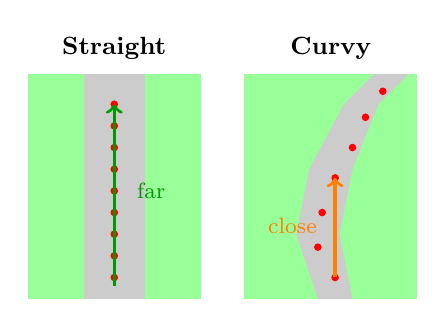
\begin{tikzpicture}[scale=0.55]
    % Straight road
    \node[font=\small\bfseries] at (0, 5.8) {Straight};
    \draw[fill=green!40, draw=none] (-2,0) rectangle (2,5.2);
    \draw[fill=gray!40, draw=none] (-0.7,0) rectangle (0.7,5.2);
    \foreach \y in {0.5,1,1.5,2,2.5,3,3.5,4,4.5} {
        \fill[red] (0, \y) circle (2.5pt);
    }
    \draw[->, very thick, green!60!black] (0, 0.3) -- (0, 4.5);
    \node[right, font=\footnotesize, green!60!black] at (0.3, 2.5) {far};

    % Curvy road
    \begin{scope}[xshift=5cm]
    \node[font=\small\bfseries] at (0, 5.8) {Curvy};
    \draw[fill=green!40, draw=none] (-2,0) rectangle (2,5.2);
    \draw[fill=gray!40, draw=none]
        (-0.3,0) -- (-0.8,1.5) -- (-0.5,3) -- (0.3,4.5) -- (1.0,5.2)
        -- (1.8,5.2) -- (1.1,4.5) -- (0.5,3) -- (0.2,1.5) -- (0.5,0) -- cycle;
    \fill[red] (0.1, 0.5) circle (2.5pt);
    \fill[red] (-0.3, 1.2) circle (2.5pt);
    \fill[red] (-0.2, 2.0) circle (2.5pt);
    \fill[red] (0.1, 2.8) circle (2.5pt);
    \fill[red] (0.5, 3.5) circle (2.5pt);
    \fill[red] (0.8, 4.2) circle (2.5pt);
    \fill[red] (1.2, 4.8) circle (2.5pt);
    \draw[->, very thick, orange] (0.1, 0.5) -- (0.1, 2.8);
    \node[left, font=\footnotesize, orange] at (-0.1, 1.7) {close};
    \end{scope}
\end{tikzpicture}
\end{column}
\end{columns}
\end{frame}

% ==========================================================
% SLIDE 5c: Classical — Steering & Speed Control
% ==========================================================
\begin{frame}[shrink=5]{Classical Agent --- Steering \& Speed Control}
\begin{columns}[T]
\begin{column}{0.55\textwidth}
\textbf{Steering:}
\begin{itemize}\setlength\itemsep{0em}
    \item Compute angle from car to target point
    \item Multiply by \textbf{3.4} $\to$ steering command
    \item Bigger angle = sharper turn
\end{itemize}

\vspace{0.3em}
\textbf{Speed control:}
\begin{itemize}\setlength\itemsep{0em}
    \item Angle $<$ 0.6 rad ($\sim$34\textdegree): gas slides 0.35 $\to$ 0.1
    \item Angle $\geq$ 0.6 rad: gas = 0.1, brake = 0.1
    \item No velocity sensor --- fixed throttle schedule
\end{itemize}
\end{column}
\begin{column}{0.42\textwidth}
\centering
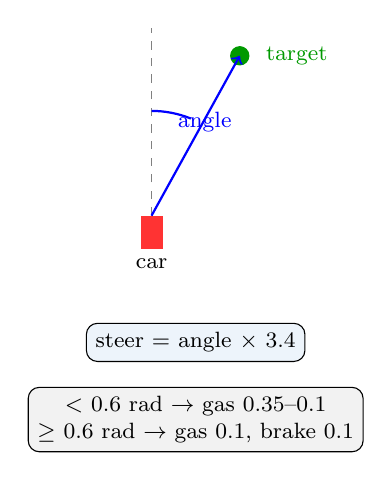
\begin{tikzpicture}[scale=0.7]
    % Car — shifted up
    \fill[red!80] (0, 1.5) rectangle (0.4, 2.1);
    \node[below, font=\footnotesize] at (0.2, 1.5) {car};

    % Target point
    \fill[green!60!black] (1.8, 5.0) circle (5pt);
    \node[right, font=\footnotesize, green!60!black] at (2.1, 5.0) {target};

    % Angle arc
    \draw[dashed, gray] (0.2, 2.1) -- (0.2, 5.5);
    \draw[->, thick, blue] (0.2, 2.1) -- (1.8, 5.0);
    \draw[thick, blue] (0.2, 4.0) arc (90:68:1.9);
    \node[right, font=\footnotesize, blue] at (0.5, 3.8) {angle};

    % Formula — well below car
    \node[draw, rounded corners, fill=classical!10, font=\footnotesize, align=center]
        at (1.0, -0.2) {steer = angle $\times$ 3.4};

    % Speed diagram — spaced below formula
    \node[draw, rounded corners, fill=gray!10, font=\footnotesize, align=center]
        at (1.0, -1.6) {
        $<$ 0.6 rad $\to$ gas 0.35--0.1\\
        $\geq$ 0.6 rad $\to$ gas 0.1, brake 0.1
    };
\end{tikzpicture}
\end{column}
\end{columns}
\end{frame}

% ==========================================================
% SLIDE 6: Classical Tuning Journey
% ==========================================================
\begin{frame}{Classical Agent --- Tuning Journey}
\centering
{\small
\begin{tabular}{clrrl}
\toprule
\# & Change & Mean & Good$\geq$700 & Notes \\
\midrule
0 & Initial config & 141 & --- & seed 0 only \\
3 & First full sweep (seeds 0--9) & 502 & 4 & real baseline \\
5 & + adaptive lookahead + gain 3.4 & 602 & 6 & \\
6 & + stall-trap fix & 751 & 9 & seeds 5,6 recovered \\
7 & + aim-only-ahead check & \textbf{786} & \textbf{9} & seed 2 fixed \\
\bottomrule
\end{tabular}
}

\vspace{0.4em}
{\small
\textbf{Bug \#1 --- Stall trap:} car braked to full stop on sharp turns, sat there forever.
Fix: keep gas $\geq$ 0.1. \quad Seed 5: 207 $\to$ 741

\vspace{0.2em}
\textbf{Bug \#2 --- T-junction:} two crossing road segments $\to$ average aim lands in grass.
Fix: only aim at road \textit{ahead}. \quad Seed 2: 120 $\to$ 470
}
\end{frame}

% ==========================================================
% SLIDE: DL Agent --- Overview
% ==========================================================
\begin{frame}{DL Agent --- Overview}
\begin{columns}[T]
\begin{column}{0.52\textwidth}
{\small Instead of hand-written rules, a neural network learns everything from scratch by playing the game millions of times.}

\vspace{0.3em}
\begin{enumerate}\setlength\itemsep{0.2em}
    \item \textbf{Input} --- last 4 frames stacked (12 channels)
    \item \textbf{CNN body} --- 3 conv layers extract visual features (shared)
    \item \textbf{Policy head} --- outputs steer, gas, brake
    \item \textbf{Value head} --- predicts future reward (training only)
\end{enumerate}

\vspace{0.3em}
{\small No perception code, no planner, no controller --- the CNN replaces \textit{all three}.}
\end{column}
\begin{column}{0.45\textwidth}
\centering
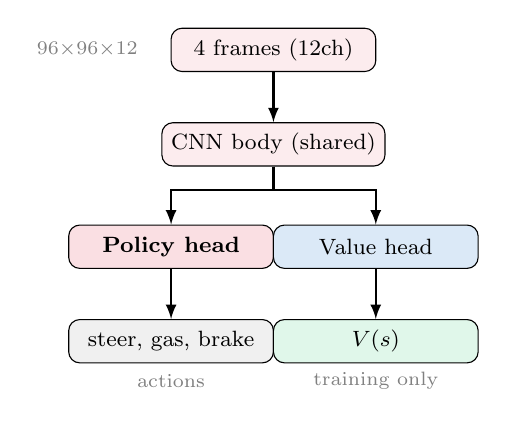
\begin{tikzpicture}[
    block/.style={draw, rounded corners=4pt, minimum width=2.6cm, minimum height=0.55cm, align=center, font=\footnotesize},
    >=latex,
]
    % Input
    \node[block, fill=dlred!12] (inp) at (0, 4.8) {4 frames (12ch)};
    \node[left, font=\scriptsize, color=gray] at (-1.6, 4.8) {96$\times$96$\times$12};

    % CNN body
    \node[block, fill=dlred!12] (cnn) at (0, 3.6) {CNN body (shared)};

    % Two heads
    \node[block, fill=dlred!20] (pol) at (-1.3, 2.3) {\textbf{Policy head}};
    \node[block, fill=classical!20] (val) at (1.3, 2.3) {Value head};

    % Outputs
    \node[block, fill=gray!12] (act) at (-1.3, 1.1) {steer, gas, brake};
    \node[block, fill=goodgreen!15] (vout) at (1.3, 1.1) {$V(s)$};

    % Arrows — clean straight lines
    \draw[->, thick] (inp) -- (cnn);
    \draw[->, thick] (cnn.south) -- ++(0, -0.3) -| (pol.north);
    \draw[->, thick] (cnn.south) -- ++(0, -0.3) -| (val.north);
    \draw[->, thick] (pol) -- (act);
    \draw[->, thick] (val) -- (vout);

    % Labels
    \node[font=\scriptsize, color=gray] at (-1.3, 0.6) {actions};
    \node[font=\scriptsize, color=gray] at (1.3, 0.6) {training only};
\end{tikzpicture}
\end{column}
\end{columns}
\end{frame}

% ==========================================================
% SLIDE: DL Agent --- How PPO Works
% ==========================================================
\begin{frame}{DL Agent --- PPO Training Loop}
\begin{columns}[T]
\begin{column}{0.40\textwidth}
\centering
\vspace{0.5em}
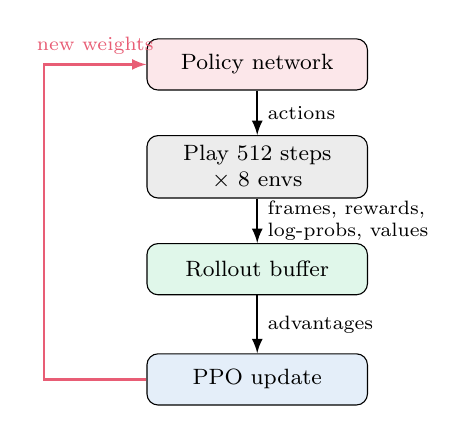
\begin{tikzpicture}[
    block/.style={draw, rounded corners=4pt, minimum width=2.8cm, minimum height=0.65cm, align=center, font=\footnotesize},
    >=latex,
]
    \node[block, fill=dlred!15] (pol) at (0, 4) {Policy network};
    \node[block, fill=gray!15] (env) at (0, 2.7) {Play 512 steps\\$\times$ 8 envs};
    \node[block, fill=goodgreen!15] (buf) at (0, 1.4) {Rollout buffer};
    \node[block, fill=classical!15] (upd) at (0, 0) {PPO update};

    \draw[->, thick] (pol) -- node[right, font=\scriptsize] {actions} (env);
    \draw[->, thick] (env) -- node[right, font=\scriptsize, align=left] {frames, rewards,\\log-probs, values} (buf);
    \draw[->, thick] (buf) -- node[right, font=\scriptsize] {advantages} (upd);
    \draw[->, thick, dlred] (upd.west) -- ++(-1.3, 0) |- node[near end, above, font=\scriptsize] {new weights} (pol.west);
\end{tikzpicture}

\vspace{0.3em}
{\scriptsize Repeat ${\sim}$4000 cycles $=$ 2M steps}
\end{column}
\begin{column}{0.57\textwidth}
\vspace{0.5em}
\textbf{Each cycle:}
\begin{enumerate}\setlength\itemsep{0.4em}
    \item Policy plays 512 steps on 8 parallel tracks
    \item Store every (frame, action, reward, log-prob, value prediction) in a buffer
    \item Compute \textbf{advantages} per step:\\
          {\small actual discounted return $-$ value prediction\\
          $=$ ``how much better/worse was this action than expected?''}
    \item Update the network weights (next slide)
    \item \textbf{Discard buffer}, collect fresh data with the improved policy
\end{enumerate}
\end{column}
\end{columns}
\end{frame}

% ==========================================================
% SLIDE: DL Agent --- PPO Loss
% ==========================================================
\begin{frame}{DL Agent --- PPO Loss Function}
\centering
\vspace{0.3em}
{\large $L = L_{\text{policy}} + 0.5 \cdot L_{\text{value}} - 0.01 \cdot H$}

\vspace{0.6em}
\begin{columns}[T]
\begin{column}{0.32\textwidth}
\centering
\textbf{\textcolor{dlred}{$L_{\text{policy}}$}}\\[0.3em]
{\small
Make good actions more likely, bad actions less likely.

\vspace{0.3em}
\textbf{Clipped} (range = 0.2): policy can't change too much per update.
This is the ``proximal'' in PPO.
}
\end{column}
\begin{column}{0.32\textwidth}
\centering
\textbf{\textcolor{classical}{$L_{\text{value}}$}}\\[0.3em]
{\small
MSE between value head's prediction and actual return.

\vspace{0.3em}
Better value predictions $\to$ better advantage estimates next cycle.
}
\end{column}
\begin{column}{0.32\textwidth}
\centering
\textbf{\textcolor{goodgreen}{$H$ (entropy)}}\\[0.3em]
{\small
Rewards the policy for staying uncertain --- keeps exploring instead of committing too early to a mediocre strategy.
}
\end{column}
\end{columns}

\vspace{0.6em}
{\small One combined loss, one backprop through entire network (CNN body + both heads).\\
10 epochs per buffer (mini-batches of 128), then discard and collect fresh data.}
\end{frame}

% ==========================================================
% SLIDE: DL Agent --- Frame Stacking
% ==========================================================
\begin{frame}{DL Agent --- Why Frame Stacking?}
\centering
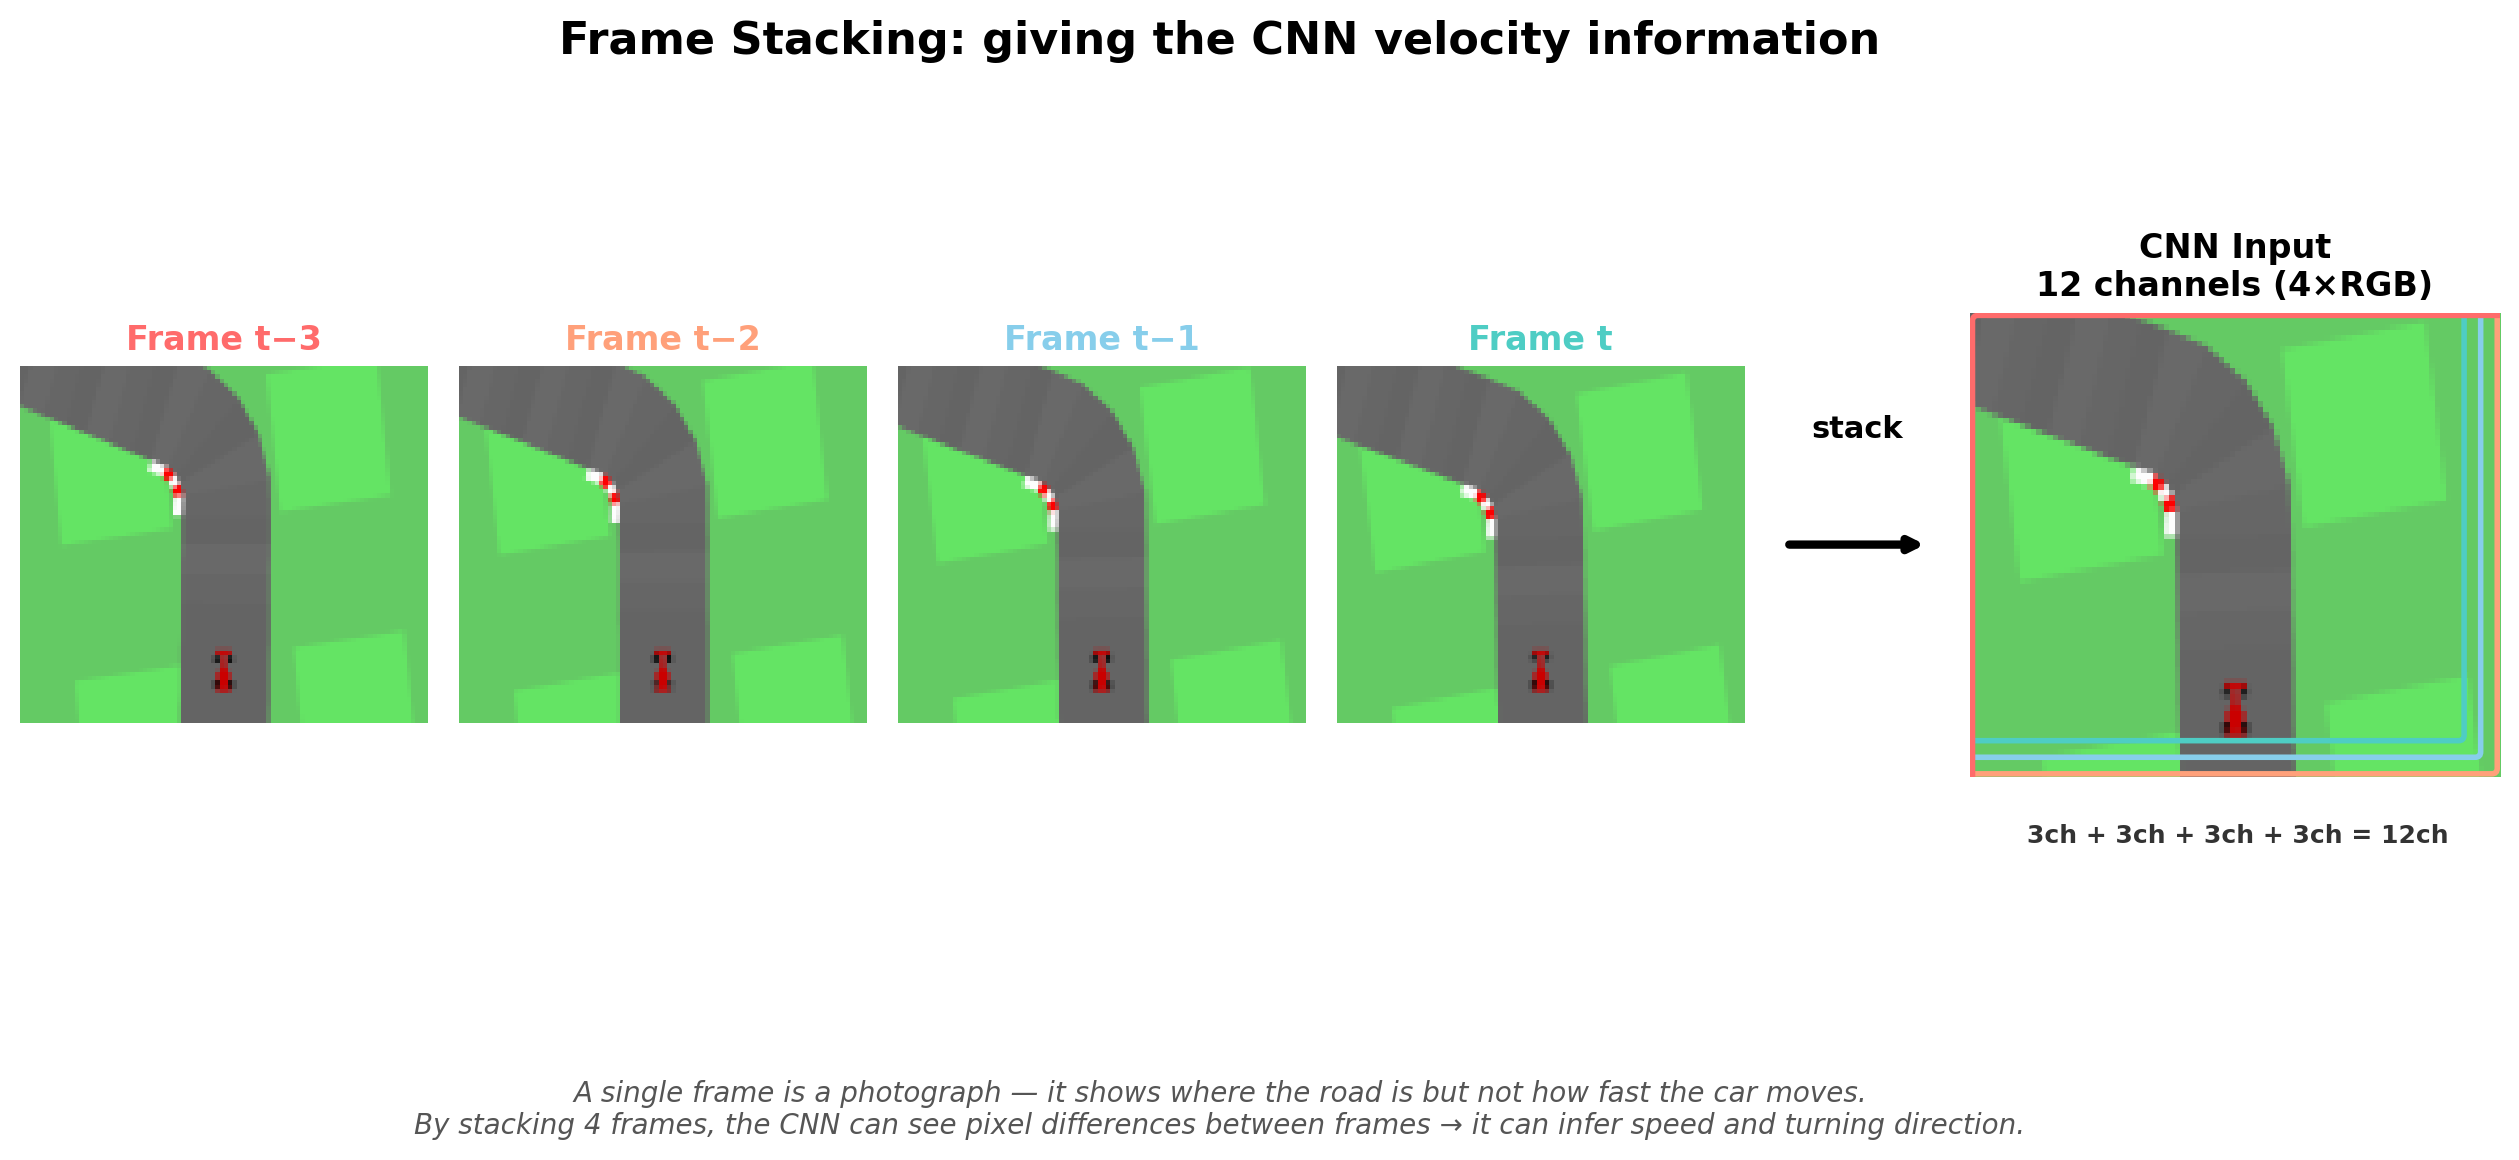
\includegraphics[width=0.75\textwidth]{frame_stacking.png}

\vspace{0.2em}
{\small
\textbf{Problem:} A single frame shows \textit{where} the road is but not \textit{how fast} the car moves.\\
\textbf{Fix:} Stack 4 frames (12 channels). CNN sees pixel differences $\to$ infers speed and direction.\\[0.2em]
Without frame stacking: mean 402. \quad With frame stacking: mean \textbf{855.8}, 3 full laps.
}
\end{frame}

% ==========================================================
% SLIDE: DL Agent --- Training Results
% ==========================================================
\begin{frame}{DL Agent --- Training Results}
\begin{columns}[T]
\begin{column}{0.55\textwidth}
\textbf{Training config:}
\begin{itemize}\setlength\itemsep{0.2em}
    \item 2M steps, 8 parallel envs
    \item Kaggle T4 GPU, $\sim$6 hours
    \item lr = $10^{-4}$, batch = 128, 10 epochs/update
    \item Clip range = 0.2 (limits how much the policy changes per update)
\end{itemize}

\vspace{0.5em}
{\small
\begin{tabular}{clrr}
\toprule
\# & Config & Mean & Laps \\
\midrule
1 & No frame stack, 500K & 197 & 0 \\
2 & No frame stack, 2M & 402 & 0 \\
\textbf{3} & \textbf{+ frame stack, 2M} & \textbf{855.8} & \textbf{3} \\
\bottomrule
\end{tabular}
}
\end{column}
\begin{column}{0.42\textwidth}
\vspace{1em}
\textbf{What the CNN learned:}
\begin{itemize}\setlength\itemsep{0.3em}
    \item Steer toward road center (like classical)
    \item \textbf{Brake before sharp turns} --- something classical can't do (no velocity info)
    \item Recover from small mistakes by counter-steering
    \item Handle T-junctions without confusion (no averaging trick needed)
\end{itemize}
\end{column}
\end{columns}
\end{frame}

% ==========================================================
% SLIDE: Demo
% ==========================================================
\begin{frame}{Demo: Side-by-Side Driving (seed 3)}
\begin{columns}[T]
\begin{column}{0.55\textwidth}
\centering
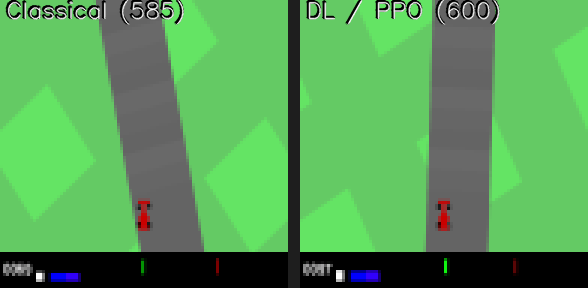
\includegraphics[width=\textwidth]{demo_still.png}

\vspace{0.3em}
{\scriptsize\color{gray} Play visuals/demo\_driving.mp4 during presentation}
\end{column}
\begin{column}{0.42\textwidth}
\vspace{0.5em}
{\small Same track, same start. Both complete the lap.}

\vspace{0.6em}
\textbf{Watch for:}
{\small
\begin{itemize}\setlength\itemsep{0.2em}
    \item \textcolor{dlred}{\textbf{DL}} brakes before sharp turns (learned from stacked frames)
    \item \textcolor{classical}{\textbf{Classical}} holds fixed throttle (no velocity sensor)
    \item DL recovers smoother from small deviations
\end{itemize}
}
\end{column}
\end{columns}
\end{frame}

% ==========================================================
% SLIDE 9: Head-to-Head Bar Chart
% ==========================================================
\begin{frame}{Head-to-Head: Classical vs DL (10 random tracks)}
\centering
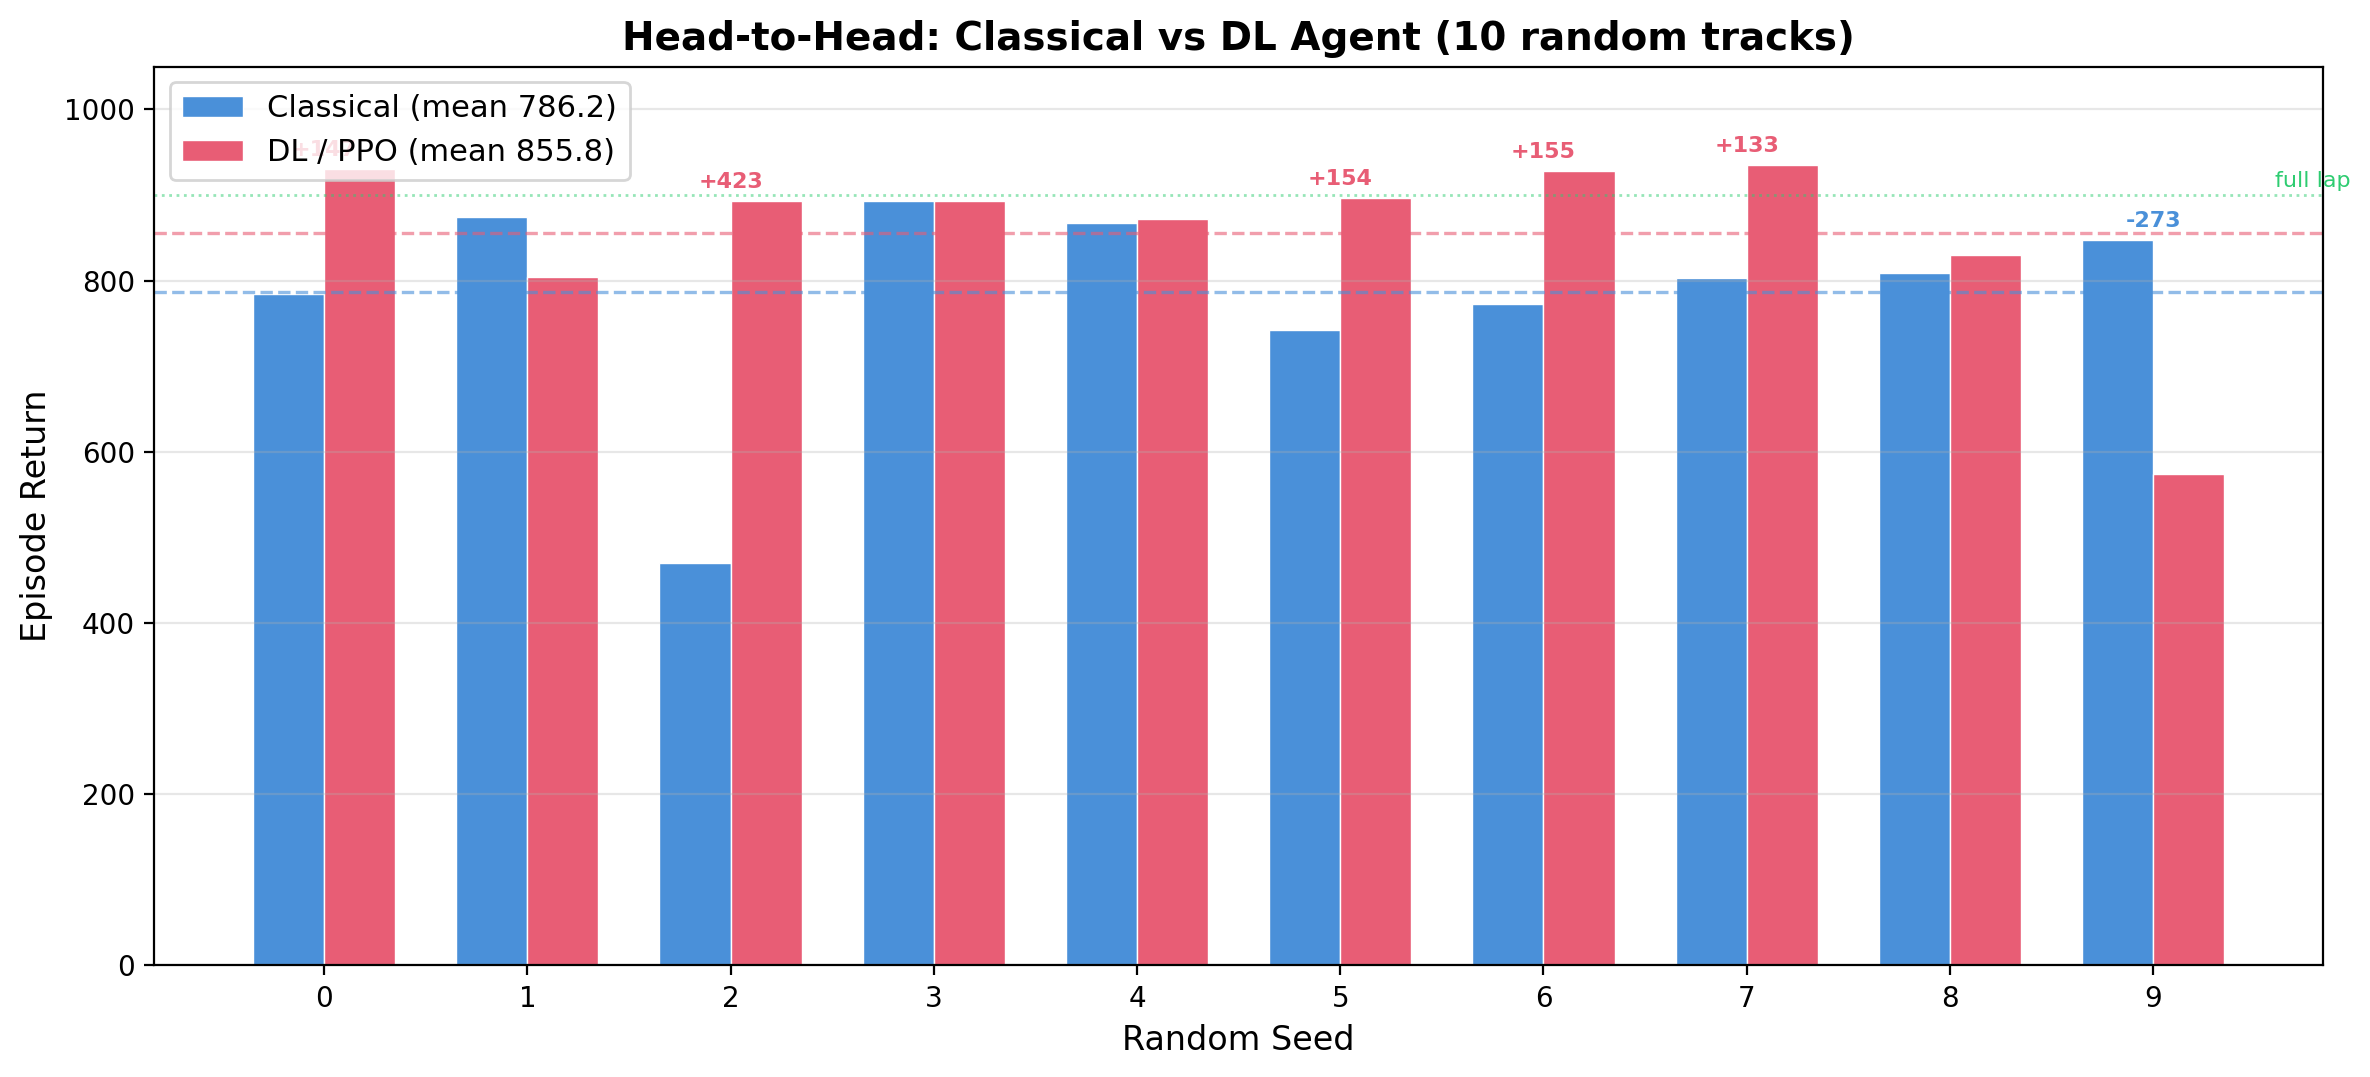
\includegraphics[width=0.82\textwidth]{bar_chart.png}

\vspace{0.2em}
{\small
\textcolor{dlred}{\textbf{DL wins:}} mean 855.8 vs 786.2, seed 2: +423, 3 full laps vs 0
\hspace{1.5em}
\textcolor{classical}{\textbf{Classical wins:}} seed 9: 847 vs 574
}
\end{frame}

% ==========================================================
% SLIDE 10: Tradeoffs Table
% ==========================================================
\begin{frame}{The Tradeoffs}
\centering
\begin{tabular}{lcc}
\toprule
 & \textcolor{classical}{\textbf{Classical}} & \textcolor{dlred}{\textbf{DL / PPO}} \\
\midrule
Mean score & 786.2 & \textbf{855.8} \\
Full laps ($\geq$900) & 0 / 10 & \textbf{3 / 10} \\
Training time & \textbf{0} (hand-tuned) & $\sim$6h on T4 GPU \\
Engineering time & $\sim$4h of tuning & $\sim$20 min code + waiting \\
Interpretability & \textbf{Full} --- every rule is visible & None --- black box \\
Speed awareness & No (fixed throttle) & \textbf{Yes} (learned from frames) \\
Failure mode & Predictable: stalls, grass & Unpredictable: just fails \\
ms / frame & \textbf{4.68} & 5.06 \\
\bottomrule
\end{tabular}
\end{frame}

% ==========================================================
% SLIDE 11: Robustness --- What is Gaussian Pixel Noise?
% ==========================================================
\begin{frame}{Robustness Test 1: Gaussian Pixel Noise}
\textbf{What is it?}\\[0.3em]
Add random static to every pixel --- like a grainy camera.
Each pixel gets bumped by a random amount; $\sigma$ controls how strong.
At $\sigma$=50, the image looks like a TV with bad reception.

\vspace{0.8em}
\textbf{Why test this?}\\[0.3em]
Real cameras have sensor noise, lighting changes, dust.
An agent that only works on clean images is fragile.

\vspace{0.8em}
\textbf{Question:} Which agent handles noise better --- the one with hard-coded color rules, or the one that learned from pixels?
\end{frame}

% ==========================================================
% SLIDE 12: Robustness --- Noise Results
% ==========================================================
\begin{frame}{Noise Results: DL Survives, Classical Collapses}
\begin{columns}[T]
\begin{column}{0.55\textwidth}
\centering
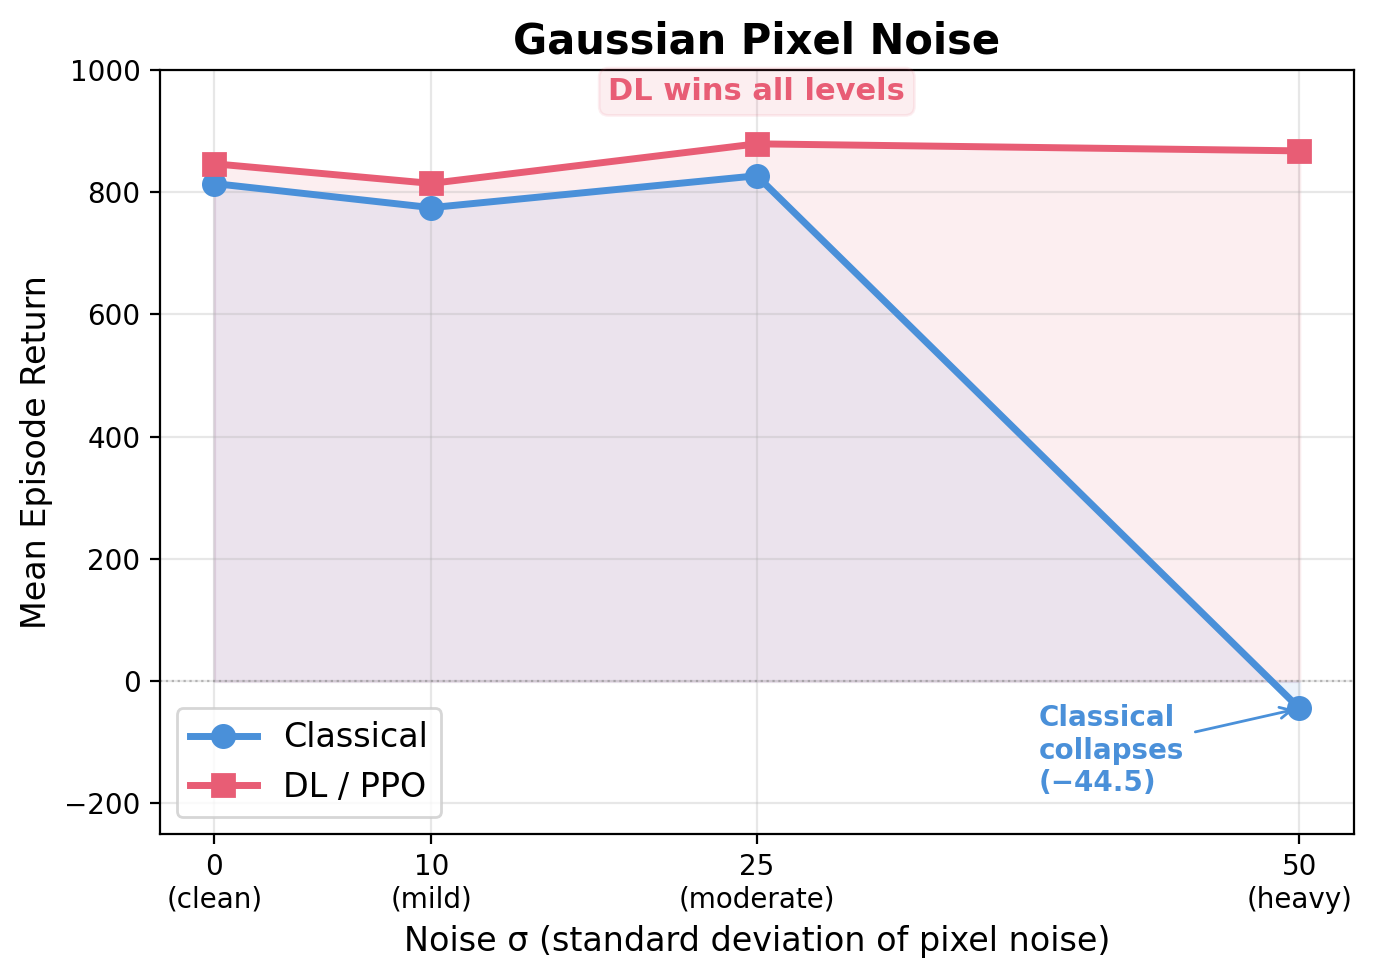
\includegraphics[width=\textwidth]{robustness_noise.png}
\end{column}
\begin{column}{0.42\textwidth}
\vspace{1em}
\textbf{\textcolor{classical}{Classical collapses}} at $\sigma$=50:

{\small The road-finding rule uses a hard cutoff ---
``if color intensity $\leq$ 60, it's road.''
Noise bumps pixels across that boundary $\to$ road mask flickers.}

\vspace{0.5em}
\textbf{\textcolor{dlred}{DL survives:}}

{\small CNN filters average over small patches ---
random noise cancels out within each 3$\times$3 window.}
\end{column}
\end{columns}
\end{frame}

% ==========================================================
% SLIDE 13: Robustness --- What is Hue Shift?
% ==========================================================
\begin{frame}{Robustness Test 2: Hue Shift (Recolored Track)}
\textbf{What is it?}\\[0.3em]
Rotate every pixel's color by a fixed amount --- the gray road might become blue,
the green grass might become purple.
The shapes and brightness stay identical, only the colors change.

\vspace{0.8em}
\textbf{Why test this?}\\[0.3em]
Different environments have different colors (desert = tan, snow = white).
A robust agent shouldn't depend on memorizing one specific palette.

\vspace{0.8em}
\textbf{Question:} Which agent handles recoloring better --- the one that checks brightness, or the one that learned from specific colors?
\end{frame}

% ==========================================================
% SLIDE 14: Robustness --- Hue Shift Results
% ==========================================================
\begin{frame}{Hue Shift Results: Classical Survives, DL Collapses}
\begin{columns}[T]
\begin{column}{0.55\textwidth}
\centering
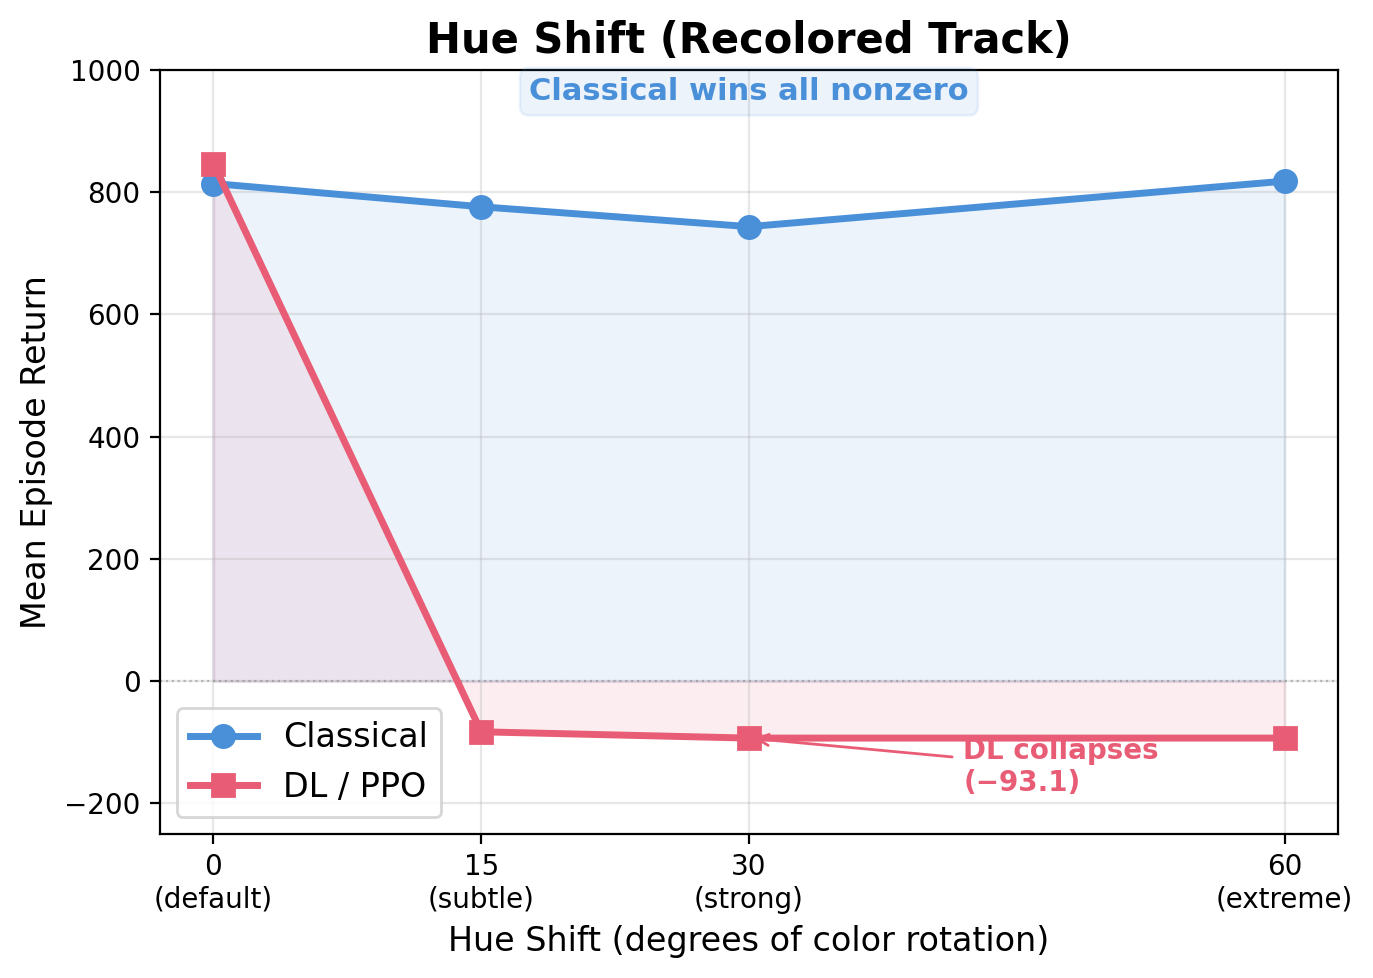
\includegraphics[width=\textwidth]{robustness_hue.png}
\end{column}
\begin{column}{0.42\textwidth}
\vspace{1em}
\textbf{\textcolor{dlred}{DL collapses}} at shift 15+:

{\small The CNN memorized the exact colors from 2M training frames.
It has never seen a blue road --- those pixels are outside its
training distribution $\to$ random actions.}

\vspace{0.5em}
\textbf{\textcolor{classical}{Classical survives:}}

{\small It checks brightness and color intensity,
but ignores \textit{which} color the road is. Rotating the hue doesn't
change the brightness.}
\end{column}
\end{columns}
\end{frame}

% ==========================================================
% SLIDE: Lessons Learned
% ==========================================================
\begin{frame}{Lessons Learned}
{\footnotesize
\begin{enumerate}\setlength\itemsep{0.25em}
    \item \textbf{\textcolor{dlred}{DL is more adaptive.}} Point it at new data $\to$ it adapts. Good when the task is complex or hard to describe in rules.

    \item \textbf{\textcolor{classical}{Classical needs handcrafted tuning.}} Feasible here (3 bugs, 4h). On a complex task --- lane changes, pedestrians, weather --- the rule count explodes.

    \item \textbf{\textcolor{classical}{Classical is fully interpretable.}} Every decision is a named constant. When DL fails, you get \textit{no} explanation.

    \item \textbf{Neither is strictly better.} Failure modes are complementary: DL survives noise but breaks under hue shift; classical is the opposite.

    \item \textbf{Training cost $\neq$ engineering cost.} DL = 6h GPU + 20 min code. Classical = 0 training + 4h tuning. You pay either way.
\end{enumerate}
}
\end{frame}

% ==========================================================
% SLIDE: Thank You
% ==========================================================
\begin{frame}{}
\centering
\vspace{2em}
{\Huge\bfseries Thank You}

\vspace{1.5em}
{\large
\begin{tabular}{rl}
Code: & \texttt{github.com/.../Agents\_comparison} \\
Task: & Gymnasium CarRacing-v3 \\
Classical: & HSV threshold + adaptive lookahead + P-control \\
DL: & PPO + CnnPolicy + 4-frame stack (SB3) \\
\end{tabular}
}

\vspace{1.5em}
{\color{gray}\small Yue Wu --- April 2026}
\end{frame}

\end{document}
